\chapter{热化中的反常动力学}\label{chap:scar}

孤立系统的热化在理解宏观系统的量子统计描述中扮演重要的角色。对于仅有局域相互作用的哈密顿量,本征热化假说被提出用来给出孤立系统热化的解释。目前为止对此假说的论证主要集中于数值模拟。但是人们目前还不严格清楚其适用的范围。有趣的的是在一些特殊体系中,本征热化假说完全失效,称为强违背本征热化假说体系,其中以量子可积系统与多体局域化系统最为典型。随着认识的不断加强,依赖于初态选取的弱违背本征热化假说体系被发现:从某些初态出发会热化,但是从某些初态出发则不会热化。在本章中,我们选择固定的初态如$|Z_2\rangle$出发,探索整个参数区间下带有纵场的横场伊辛模型的热化相图,并讨论出现的不同区域及其背后的物理解释。我们在第一节中给出此研究的动机,第二节中讨论涉及的模型和方法,在第三节中针对得到的相图分析热化的发生与否,在最后一节我们总结目前的结果并做简要的小结。

\section{引言}
在热力学平衡态的角度,量子统计力学给出了宏观物体的热力学描述。仅用几个参数就可以描述处于热力学平衡态的宏观数目自由度的体系。而量子统计力学中一个关键原理即是等概率原理——具有相同能量的微观量子态在热力学平衡态分布中出现的几率相同。基于此原理,我们引入微正则系综来描述平衡态分布,为了与实验体系方便比较,我们又引入了在热力学极限下与之等价的正则系综与巨正则系综。但是在另一个角度,根据量子力学基本定律,我们知道孤立量子体系的演化为幺正的。如果我们准备一个孤立系统处于初态$|\psi(t=0)\rangle$,初态在不同本征态上的投影几率为$\langle E_\alpha|\psi(t=0)\rangle$,这一几率在幺正时间演化下是不变的。对于一个系统的长时间平均测量,其观测值似乎在初态决定的时候就已经决定了,看似是初态依赖的,这与统计力学中假设的时间平均等价于等概率系综平均乍一看是矛盾的。为了解决这一矛盾,Srednicki\cite{Srednicki1994chaos}与Deutsch\cite{Deutsch1991quantum}分别独立地提出了本征热化假说(ETH),其核心思想为当我们观测一个孤立系统的局域可观测量时,系统的剩余部分作为这个局域自由度的热库,这一热接触的温度由系统总的能量给出。这一假说在后续很多体系的数值试验中得到验证。具有很强的普适性,局域算符的可观测量仅由能量决定。更加形式化的讨论以及数值证据可以参见我们第一章中给出的介绍。但大自然总是奇妙的,这一假说很快就被发现在某些体系里面完全失效,其中以量子可积系统\cite{kinoshita2006quantum,Rigol2007Relaxation,Calabrese2011Quantum,essler2016quench,vidmar2016generalized}与多体局域化系统最为典型\cite{basko2006metal,Serbyn2013local,Huse2014Phenomenology},其完全失效的原因目前仍没有确切定论,这种体系被称为完全违背本征热化假说体系。

符合本征热化假说与完全违背本征热化假说是两个极端。很快介于两个极端的弱违背本征热化假说系统被发现。典型的例子就是量子多体伤痕。这一现象最早发现于冷原子中里德堡原子平台\cite{bernien2017probing}。在一维原子链中,每个格点上里德堡原子近似为二能级体系,原子间的库伦相互作用禁止相邻的两个原子处于二能级中的里德堡激发态,可以用PXP哈密顿量来描述。该实验在$|Z_2\rangle$初态出发的动力学中发现了局域算符反常的长时间震荡行为,并且其时间平均值并不等于吉布斯系综所预测的热力学平均值。
这一实验很快地激发了相关的理论研究\cite{turner2018weak,Turner2018quantum,Ho2019periodic,Choi2019emergent,Michailidis2020slow,serbyn2021quantum,Yao2022quantum},这一反常动力学来自于PXP哈密顿量中涌现出的近似封闭的子希尔伯特空间。数值严格对角化的结果给出这一子空间里的本征态违背本征热化假说的规律。而不在此子空间的态则服从本征热化假说。基于这一图像,严格封闭的子希尔伯特空间在不同哈密顿量中被构造出来\cite{Shiraishi2017Systematic,Moudgalya2018exact,Moudgalya2018entanglement,Khemani2020lacalization,Moudgalya2020eta,Lin2019Exact,Schecter2019weak,Mark2020unified,Mark2020eta,Pakrouski2020many,Ren2021quasi,ODea2020from},自然地这些空间里的态也违背本征热化假说。但是这些态为何存在?如何在一个哈密顿量中找到这些态?我们离这些问题的答案依然很遥远。除了量子多体伤痕,在一些格点规范模型\cite{magnifico2020real,Chanda2020confinement,Borla2020confined}和禁闭模型\cite{Nandkishore2017many,kormos2017real,Robinson2019signature,Yang2020Hilbert,Castro2020entanglement}中也有观测到这种弱本征热化假说违背的现象。其与量子多体伤痕的关系目前仍尚未明确\cite{serbyn2021quantum}。


介于服从本征热化假说与完全违背本征热化假说的中间情况还有一种叫做弱热化的现象\cite{banuls2011strong}。这是在带有纵场的横场伊辛模型中被发现的。当纵场不为零时候,该模型不再是可积的。通常来讲没有无序的不可积模型是热化的,会符合本征热化假说。但是基于张量网络模拟的结果给出,从$|Z+\rangle$出发的动力学表现出一种围绕热力学均值震荡的行为。这一震荡并不是热力学涨落,被称为弱热化现象。这一现象的一个解释由基态附近准粒子激发带来\cite{Lin2017quasiparticle}。并且这一反常行为在超导量子比特模拟中被发现\cite{Chen2021observation}。

基于上述的讨论,我们看到各种热化与非热化的现象。对于一个哈密顿量来讲,本征热化假设总归是一个很严格的要求,很容易有部分违背这一假说本征态。简单的做二分类是粗糙的。目前的研究很多是固定莫某个参数或者选取某个初态来研究。给人一种相对混乱的感觉。因此在我们本章工作中,我们基于带有纵场的横场伊辛模型,选取固定的基态$|Z_2\rangle$,在整个参数区间研究其热化的相图,以期得到一个较为全面的认识。

\section{模型与方法}
我们采用严格对角化的数值方法来研究带有纵场的横场伊辛模型,我们取$g=1,\hbar=1$。
\begin{equation}
\hat{H}_{Ising} = J\sum_{i}\hat{\sigma}^z_i\sigma^z_{i+1} + h\sum_{i}\hat{\sigma}^z_i + g\sum_i\hat{\sigma}^x_i
\label{Ising}
\end{equation}
选取周期性边界条件,选取$|\downarrow\rangle=|0\rangle$,$|\uparrow\rangle=|1\rangle$,其中$\sigma_i^{x,y,z}$为泡利算符。

\subsection{对称性}
哈密顿量拥有晶格平移对称性以及空间反演对称性。对于晶格平移对称性,我们定义平移算符$\hat{T}$:
\begin{equation}
	\hat{T} |0 \quad or \quad 1 \rangle_{i} =  |0 \quad or \quad 1 \rangle_{i+1}, i=1,2...L
\end{equation}
平移算符与哈密顿量对易:
\begin{equation}
	\hat{T}^{-1}\hat{H}_{Ising}\hat{T} = \hat{H}_{Ising}\\
\end{equation}
因此我们选取布洛赫动量态,作为晶格平移算符与哈密顿量共同本征态。布洛赫动量量子数可以取 $K_i=\frac{2\pi\cdot i}{L},i=0,1...L-1$,为动量算符$\hat{K}$的本征值,其中$\hat{K}$的定义为$\hat{T} = e^{-i\cdot\hat{\vec{K} }\cdot \vec{a}}$的生成元。

第二个全局对称性为空间反演对称性$\hat{I}$:
\begin{equation}
	\hat{I} |0 \quad or \quad 1 \rangle_{i} =  |0 \quad or \quad 1 \rangle_{L+1-i}, i=1,2...L
\end{equation}
同样地与哈密顿量对易关系为:
\begin{equation}
	\hat{I}^{-1}\hat{H}_{Ising}\hat{I} = \hat{H}_{Ising}\\
\end{equation}

不巧的是$\hat{K}$ 与 $\hat{I}$并不对易。但是在某些动量态比如$K_i=0$ 与 $K_i=\pi$子空间中,反演算符与$\hat{K}$与$\hat{I}$是对易的,此时我们可以进一步将空间划分为宇称为$+$与$-$的子空间。在做了如上块对角化之后,我们将要严格对角化的矩阵维度最大为动量宇称$KP=0+$
子空间的维度$D_{0+}=27012$。


\subsection{时间平均与系综平均}
考虑一个初态出发,系统的局域可观测量最终是否热化。我们需要将长时间平均的结果与热力学吉布斯系综平均的结果做比较。其中对于时间平均,在将对称性导致的简并考虑完毕后,体系通常情况下不再拥有简并。我们记此时子空间的本征能量与本征解为$E_\alpha$ 与 $|\alpha\rangle$:
\begin{equation}
\hat{H} |\alpha\rangle = E_\alpha |\alpha\rangle, \alpha=1,2...D
\end{equation}
其中D为考虑全局对称性块对角化之后子空间的维度。当考虑局域算符$\hat{L}$的长时间演化时,从初态$|\psi(t=0)\rangle$出发,t时刻$|\psi(t)\rangle$ 有:
\begin{equation}
|\psi(t)\rangle = e^{-i\hat{H}t}|\psi(t=0)\rangle = \sum_{\alpha=1}^D e^{-i E_\alpha t} \langle\alpha|\psi(t=0) \rangle  |\alpha\rangle
\end{equation}
时间平均为:
\begin{equation}
\begin{split}
	\bar{L}_{\infty}  &= \lim_{T\to \infty} \frac{1}{T} \int_{t_0}^{t_0+T} \langle\psi(t)|\hat{L}|\psi(t)\rangle dt \\
		\quad &=  \sum_{\alpha} \langle\alpha|\hat{L}|\alpha\rangle |\langle\alpha|\psi(t=0)\rangle|^2  +  \lim_{T\to \infty} \frac{1}{T} \int_{t_0}^{t_0+T} dt \\
		&\quad \cdot\sum_{\alpha\neq\gamma} \langle\alpha|\hat{L}|\gamma\rangle \langle\gamma|\psi(0)\rangle \langle\psi(0)|\alpha\rangle e^{-i(E_\gamma-E_\alpha)t}
\end{split}
\end{equation}
从黎曼积分定理我们知道非对角元的部分在长时间$T\to\infty$平均下贡献为零。仅剩对角元部分有贡献,此即对角系综:
\begin{equation}
	\bar{L}_{\infty} =  \sum_{\alpha} \langle\alpha|\hat{L}|\alpha\rangle |\langle\alpha|\psi(t=0)\rangle|^2  = Tr(\hat{\rho}_{DE}\hat{L}) = \bar{L}_{DE}
\end{equation}

而在另一方面,考虑吉布斯系综平均时我们有平均能量与动量定义为:
\begin{equation}
\begin{split}
 \bar{E} &= \langle\psi(t=0)|\hat{H}|\psi(t=0)\rangle \\
 \bar{K} &= \langle\psi(t=0)|\hat{K}|\psi(t=0)\rangle\\
\end{split}
\end{equation}
接着我们定义对应吉布斯系综分布:
\begin{equation}
\hat{\rho}_{th} = \frac{1}{Z}e^{-\beta\hat{H}-\lambda\hat{K}}, Z = Tr(e^{-\beta\hat{H}-\lambda\hat{K}})
\end{equation}
其中的$\beta,\lambda$由下式给定:
\begin{equation}
\begin{split}
	\bar{E} &= Tr(\hat{\rho}_{th}\hat{H} ) \\
	\bar{K} &= Tr(\hat{\rho}_{th}\hat{K})
\end{split}
\end{equation}
一旦我们得到$\beta$ 与 $\lambda$,局域算符的热力学系综期望值即为:
\begin{equation}
	\bar{L}_{th} = Tr(\hat{\rho}_{th}\hat{L})
\end{equation}

为了消除严格对角化中尺寸的效应,我们对两种平均都做了有限尺寸修正。

\section{相图与分析}
我们主要的数值模拟结果可以总结在下面的相图里面,对于固定的哈密顿量,参数为$J,h$,我们从初态$|Z_2\rangle$出发,我们考虑局域算符$\hat{L}=\hat{\sigma}_1^z\hat{\sigma}_2^z$,比对由对角系综求得的长时间平均以及正则系综平均得到吉布斯平均,比较两者之间的差值,我们画出有限尺寸修正后的结果:

%***********************************
\begin{figure}[h]
\centering
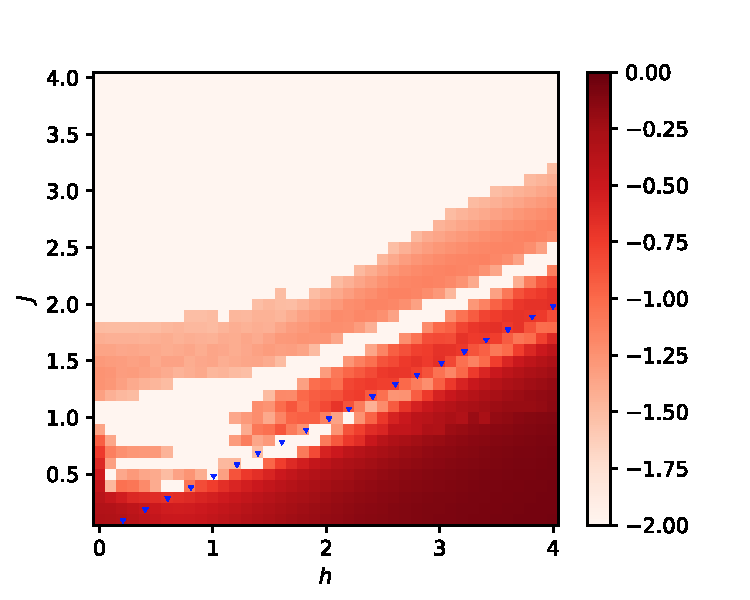
\includegraphics[width=0.7\textwidth]{./scar/scar1.pdf}
\bicaption{初态为$|Z_2\rangle$的局域算符时间平均期望值$\bar{L}_{DE}$与吉布斯系综平均期望值$\bar{L}_{th}$之差。选取不同的链长L=10,12,14,16,18,我们做有限尺寸修正,然后对两种平均的期望值做差取绝对值后再画在10为底的对数坐标下。我们选取截断$\Delta=0.03$作为临界值,绝对值低于临界值的我们在图中用白色表示。绿色的点标记$J=h$与$J=\frac{h}{2}$。}{Difference between long time average and Gibbs conanical ensemble average of local operator $\hat{L}=\hat{\sigma}_1^z\hat{\sigma}_2^z$. By choosing different lenght of chain $L=10, 12,14,16,18$, we do finite size scaling to obtain $L=\infty$ result. We choose critical difference between two averages to be $\Delta=0.03$. When $|\Delta|<0.03$, we mark as white color to represent thermalization. Green points mark special lines $J=h$ and $J=\frac{h}{2}$. }
\label{scarphasediag}
\end{figure}
%***********************************

我们将相图分为几个区域来讨论:

首先是量子多体伤痕区域,对于里德堡哈密顿量:
\begin{equation}
\begin{split}
	\hat{H}_{Rydberg}(V) &= \sum_{i=1}^{L} \hat{\sigma}_{i}^{x} + V \sum_{i}^{L} \hat{n}_i\cdot\hat{n}_{i+1} \\
	\quad &= \sum_{i=1}^{L} \hat{\sigma}_{i}^{x} + \frac{V}{4}  \sum_{i}^L \hat{\sigma}_i^z\hat{\sigma}_{i+1}^z + \frac{V}{2} \sum_i^L \hat{\sigma}_i^z  + frac{V}{4} \sum_i^L \hat{1} \\
\end{split}
\end{equation}
带入$\hat{n}_i = \frac{\hat{\sigma}_i^z+1}{2}$,我们发现如果在$\hat{H}_{Ising}(g,J,h)$中取$g=1,J=V/4,h=V/2$,则两者是等价的:
\begin{equation}
\hat{H}_{Ising}(g=1,J=\frac{V}{4},h=\frac{V}{2}) = \hat{H}_{Rydberg}(V) + C
\end{equation}

因此在带有纵场的横场伊辛模型中,如果沿着$J=h/2$这条特殊的线来看,我们就得到了里德堡哈密顿量。在$J$较大的极限下,有效模型为PXP模型,从$|Z_2\rangle$作为初态出发,会观察到局域算符期望值的持续震荡行为,而且其长时间系综平均不等于热力学系综平均,此即量子多体伤痕动力学。这是违背本征热化假说的反常动力学,在我们相图中沿着$h=2J$这条直线可以清楚的看到这一轨迹,如图~\ref{scarphasediag}~所示。。

如果我们把$J=h/2$这条线从相图里摘出,如图~\ref{scar1_2}~所示。沿着$J=h/2$这条线,当$h\ll 1$的时候,此时由于靠近单自旋极限,可以这种非热化的行为是可以期待的。当$h \gg 1$的时候,此时为PXP极限,时间平均不等于系综平均。在中间区域$h\sim 1$,我们看到由于这一极大值结构的存在,导致仅在与纵轴为0的两个交点处有局域算符的时间平均与系综平均之差为0,在其余情况下局域算符期望的时间平均不等于系综平均。

%***********************************
\begin{figure}[h]
\centering
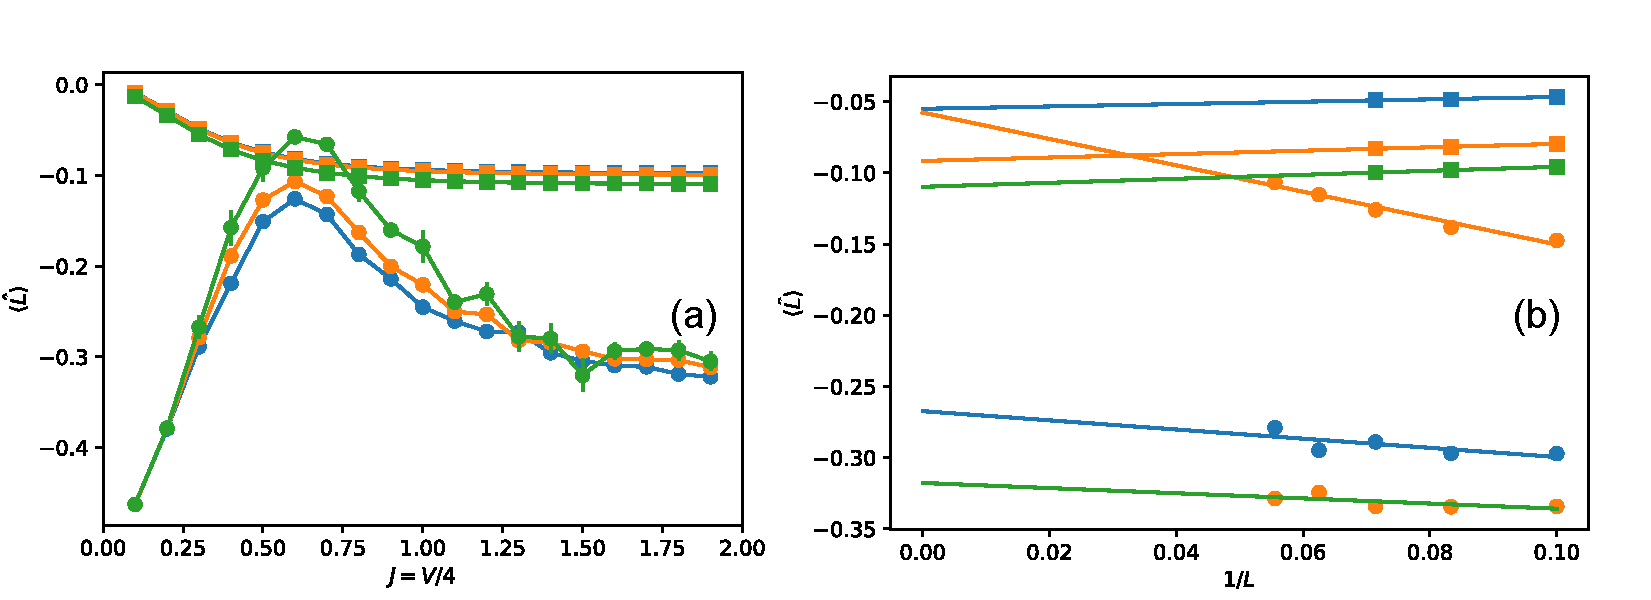
\includegraphics[width=0.7\textwidth]{./scar/scar2.pdf}
\bicaption{沿$J=h/2$特殊比例下时间平均与系综平均的差值。为有限尺寸修正之后的结果。}{Difference between time average and conanical ensemble average of local operator $\hat{L}=\hat{\sigma}_1^z\hat{\sigma}_2^z$. We show results after finite size scaling.}
\label{scar1_2}
\end{figure}
%***********************************


进一步地,如果把$J=h/2+a$这条直线摘出来看,则在J较大的区域:
\begin{equation}
\begin{split}
\hat{H}_{Ising}&= J\sum_{i}\hat{\sigma}^z_i\sigma^z_{i+1} + 2(J-a)\sum_{i}\hat{\sigma}^z_i + \sum_i\hat{\sigma}^x_i \\
\quad &= 4J\cdot( \sum_{i}^{L} \hat{n}_i\cdot\hat{n}_{i+1} + \frac{1}{4J}\sum_i\hat{\sigma}^x_i - \frac{2a}{4J} \sum_{i}\hat{\sigma}^z_i  ) + C\\
\end{split}
\end{equation}
$a$对应的纵场项会变成PXP模型中的$-2a\sum_i\sigma^z_i$,物理意义相当于在PXP模型中再加一个沿$z$方向纵场。即:
\begin{equation}
\hat{H}_{eff} = \sum_{i}^{L} \hat{P}_{i-1}\hat{\sigma}_i^x\hat{P}_{i+1} -  -2a\sum_i\hat{\sigma}^z_i 
\end{equation}
这一纵场的引入随着a的增大,首先会破坏多体伤痕动力学,使其先变为热化的行为,大约在$a_c=0.4$附近,此时多体伤痕动力学被完全破坏,这一现象在最近的研究中已经被发现\cite{Yao2022quantum},我们的结果进一步证实了这点。随着$a$继续增大,系统进入下一个区域——弱热化区域。


对于弱热化区域,此时$J \gg \frac{h}{2}$,当$g=0$时,我们有$|Z_2\rangle=|10101010...\rangle$与$|Z'_{2}\rangle=|0101001...\rangle$为系统的两个简并基态。但是着两个简并基态无法通过动力学联系起来。当$g\neq 0$时候,打开量子涨落,动力学局限在基态以及基态附近的准粒子激发附近。此时的准粒子激发主要有两类,近似为$|...00...\rangle$
与$|...11...\rangle$,对应的准粒子能量为$4J-2h$与$4J+2h$,当初态处于$|Z_2\rangle$时,此时的动力学即由准粒子决定的弱热化动力学。其震荡频率反映的是准粒子的能量,其振幅由$\sum_i \hat{\sigma}_i^x$引发的量子跃迁决定,如图~\ref{weak}~所示。

%***********************************
\begin{figure}[h]
\centering
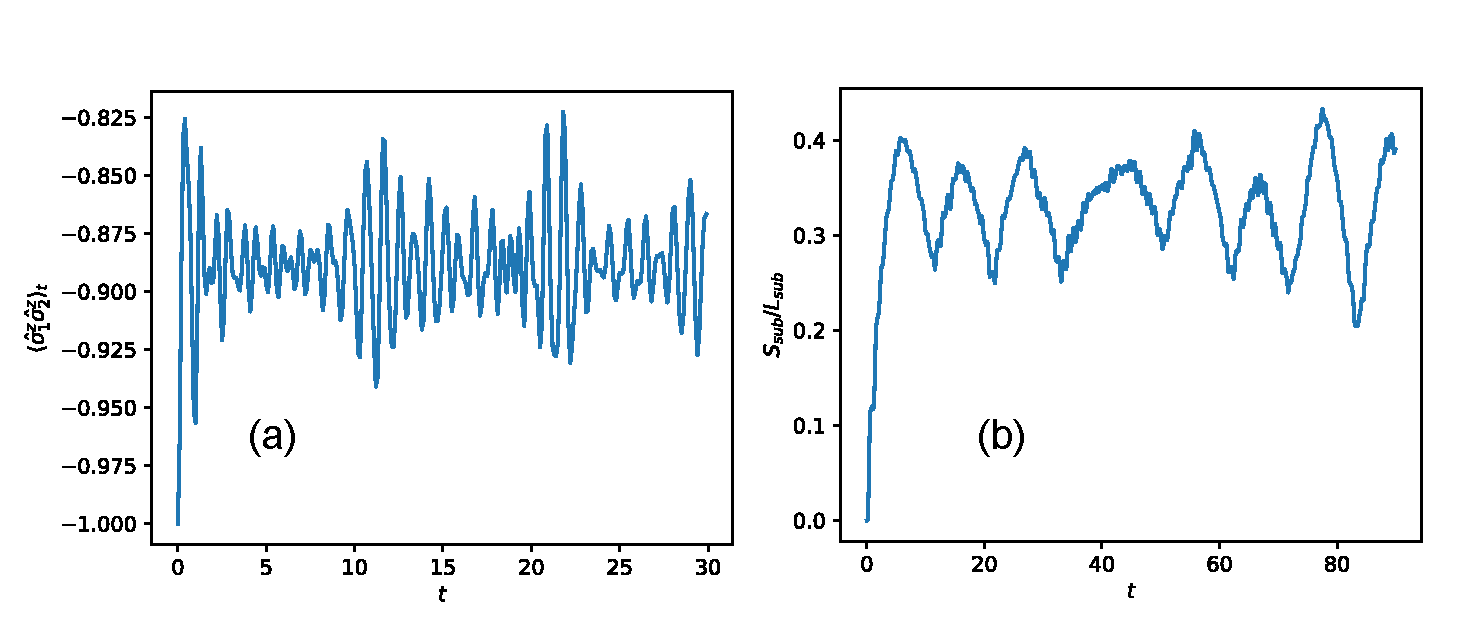
\includegraphics[width=0.8\textwidth]{./scar/scar3.pdf}
\bicaption{图(a)为$J=2.3,h=1.1$下初态为$|Z_2\rangle$的动力学演化。可以看到局域算符期望值长时间震荡的行为。图(b)为第一个格点的纠缠熵随时间的变化。我们选取此时链长为$L=16$。  }{Fig(a) for dynamics of local operator $\hat{L}=\hat{\sigma}_1^z\hat{\sigma}_2^z$ starting from$|Z_2\rangle$. Fig(b) for entanglement entropy of spin degree on first site. We choose $L=16$ for simulation. }
\label{weak}
\end{figure}
%***********************************


如果我们沿着多体伤痕区域往$h \gg J,1$的方向进入到单自旋极限区域,即相图中的右下角区域,此时系统的基态为$|Z_0\rangle$。并且在$J=0$的极限下退化到自旋之间互相解藕的区域,此区间是平凡的,对这样一个严格可解的单自旋区间,时间平均不等于正则系综平均的行为是可以预期的。

最后在中间区域$h\sim 1, J \sim 1$附近,我们的动力学结果表明此时热化仍然是很慢的,其行为类似于之前观测到的弱热化行为,与此时选取初态为$|Y-\rangle = |Y-\rangle_0 \otimes|Y-\rangle_1\otimes |Y-\rangle_2 \otimes... $的热化动力学有很大不同。
%***********************************
\begin{figure}[h]
\centering
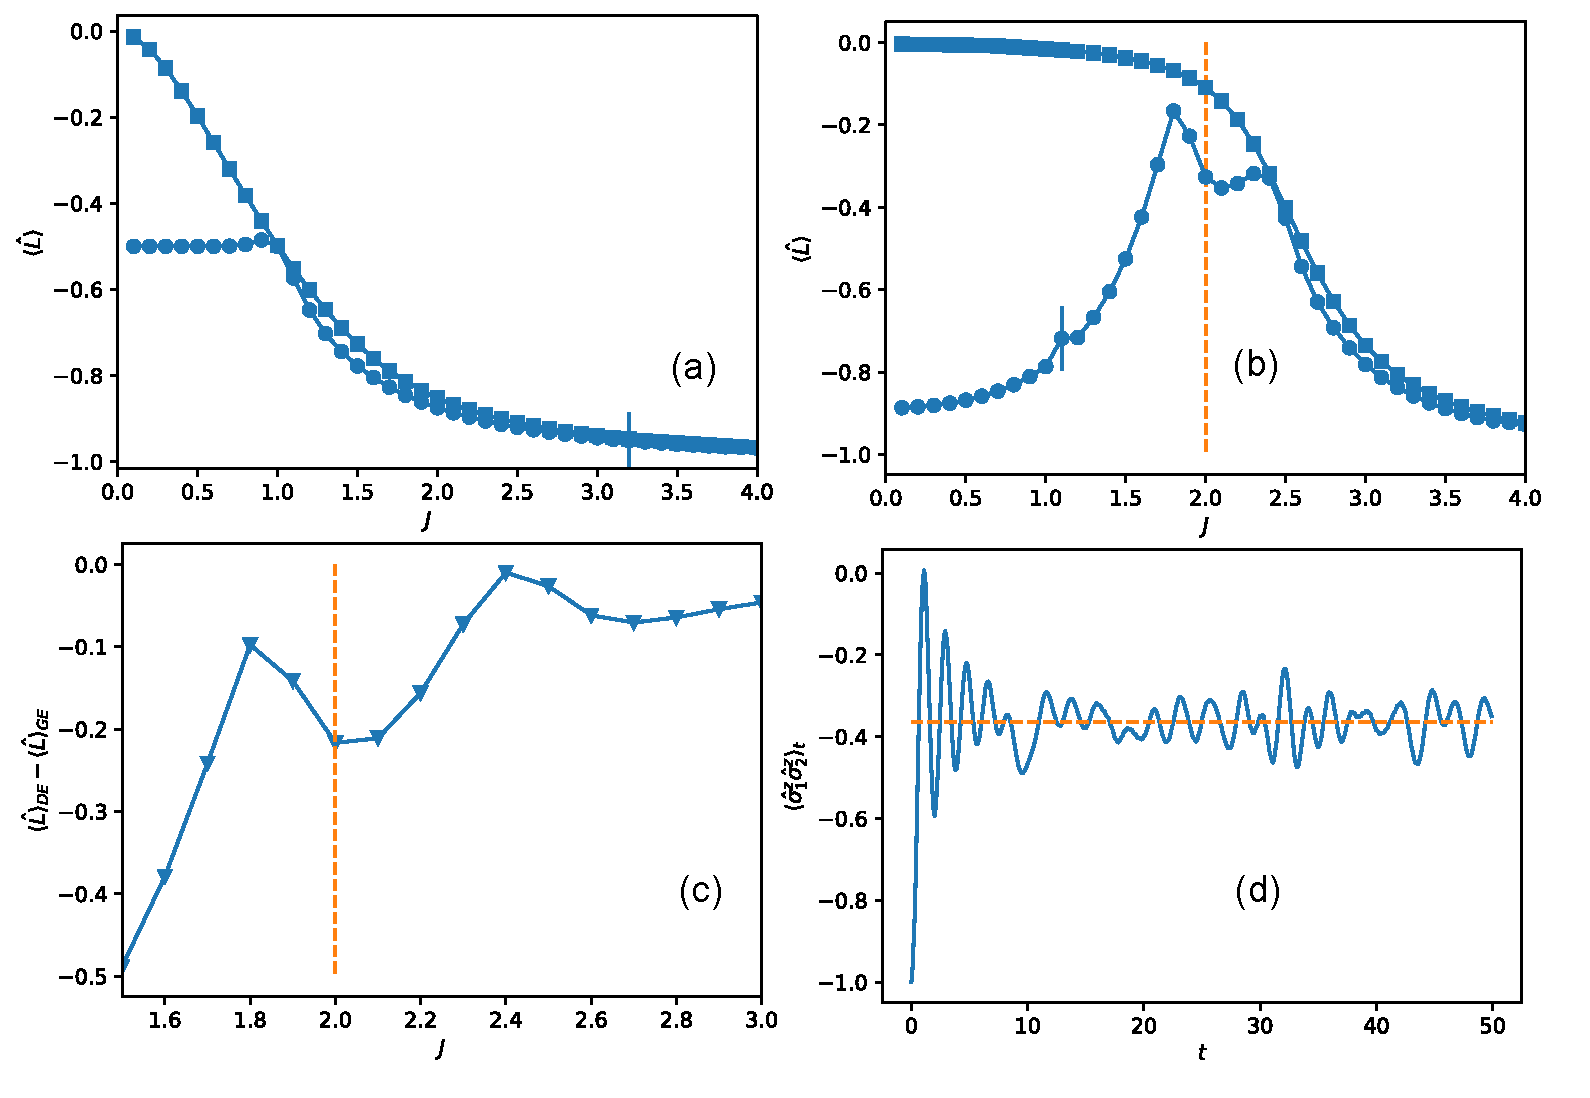
\includegraphics[width=0.8\textwidth]{./scar/scar4.pdf}
\bicaption{图(a)为$J=0.9,h=0.87$下初态为$|Z_2\rangle$的动力学演化。此时仍然可以看到局域算符期望值长时间震荡的行为。图(b)为第一个格点的约化密度矩阵随时间的变化。图(c)为$J=,h=$下初态为$|Y-\rangle$的动力学演化。此时仍然可以看到局域算符期望值长时间震荡的行为。图(d)为第一个格点的约化密度矩阵随时间的变化,初态为$|Y-\rangle$。我们选取此时链长为$L=16$。  }{Fig(a) for dynamics of local operator $\hat{L}=\hat{\sigma}_1^z\hat{\sigma}_2^z$. Fig(b) for entanglement entropy of spin degree on first site. Fig(c) for dynamics of local operator $\hat{L}=\hat{\sigma}_1^z\hat{\sigma}_2^z$. Fig(d) for entanglement entropy of spin degree on first site. We choose $L=16$ for simulation. }
\label{midweak}
\end{figure}
%***********************************




\section{小结与展望}
我们选取$|Z_2\rangle$作为初态,进行长时间动力学平均与热力学系综平均的比较,发现这一初态对应的热化相图,我们主要发现了四个区域:首先是多体伤痕区域,对应$J:h=1:2$附近,在此区域我们发现在这个强弱耦合区间内系统时间平均都不等于系综平均。随着截距的改变,对应在PXP模型下加入沿z方向的磁场,这一磁场会破坏多体伤痕动力学;在$J\gg h/2$的弱热化区域下,我们观察到了靠近基态带来的若热化动力学,并给出简单的准粒子激发解释。在$h\gg J$的区域,我们发现单自旋极限区域,此时各自选间近似孤立。最后在中间区域,我们仍然观测到了弱热化现象,并于此时强热化动力学做了对比,其中单自旋熵的震荡行为清晰地揭示了这一点。

尽管我们选取了初态为$|Z_2\rangle$,比如$|Z_0\rangle$,并讨论这些初态的不同,以期得到更加全面和系统的认识,这是在未来理解热化现象中值得进一步探索的。













